% TO DO:
% Introduction
% add coverage plot
% finish ubercal in matrix form

%% Use whichever is most appropriate for your purposes.
%%
%%\documentclass[12pt,preprint]{aastex}
%% manuscript produces a one-column, double-spaced document:
\documentclass[manuscript]{aastex}
%% preprint2 produces a double-column, single-spaced document:
%% \documentclass[preprint2]{aastex}

%% Sometimes a paper's abstract is too long to fit on the
%% title page in preprint2 mode. When that is the case,
%% use the longabstract style option.

%% \documentclass[preprint2,longabstract]{aastex}


\newcommand{\vdag}{(v)^\dagger}
\newcommand{\myemail}{holmes@mpia.de}

%% You can insert a short comment on the title page using the command below.

\slugcomment{Version 0.1}

\shorttitle{Optimizing Large Scale Surveys for Photometric Calibration}
\shortauthors{Holmes et al.}

\begin{document}

%% LaTeX will automatically break titles if they run longer than
%% one line. However, you may use \\ to force a line break if
%% you desire.

\title{Optimizing Large Scale Surveys for Photometric Calibration, \\
    The Euclid Dark Energy Mission as an Example}

%% Use \author, \affil, and the \and command to format
%% author and affiliation information.
%% Note that \email has replaced the old \authoremail command
%% from AASTeX v4.0. You can use \email to mark an email address
%% anywhere in the paper, not just in the front matter.
%% As in the title, use \\ to force line breaks.

\author{Rory Holmes\altaffilmark{1}, David W. Hogg\altaffilmark{1,2} and H.-W. Rix\altaffilmark{1}}

%% Notice that each of these authors has alternate affiliations, which
%% are identified by the \altaffilmark after each name.  Specify alternate
%% affiliation information with \altaffiltext, with one command per each
%% affiliation.

\altaffiltext{1}{Max-Planck-Institut f\"ur Astronomie, K\"onigstuhl 17, Heidelberg, 69117, Germany.}
\altaffiltext{2}{Center for Cosmology and Particle Physics, Department of Physics, New York University, 4 Washington Place, New York, NY 10003, USA.}

%% Mark off your abstract in the ``abstract'' environment. In the manuscript
%% style, abstract will output a Received/Accepted line after the
%% title and affiliation information. No date will appear since the author
%% does not have this information. The dates will be filled in by the
%% editorial office after submission.

\begin{abstract}
XX
\end{abstract}

%% Keywords should appear after the \end{abstract} command. The uncommented
%% example has been keyed in ApJ style. See the instructions to authors
%% for the journal to which you are submitting your paper to determine
%% what keyword punctuation is appropriate.

\keywords{XX, XX, XX}

\section{Introduction}
XX

\section{Sky Catalog}
We create a catalog of fake stars, based on realistic star densities, in the magnitude range $m_{min} < m < m_{max}$. We choose these limits based on the properties of single exposure of the current configuration of Euclid NISP instrument: $m_{min} = 19$, the approximate saturation limit, and $m_{max} = 22.5$, the 10$\sigma$ limit. Stars are generated with random coordinates (uniformly distributed within the sky region being investigated) and with random magnitudes distributed according to the following powerlaw:
\begin{displaymath}
\log_{10} \frac{dN}{d\Omega\,dm} = a + b\,m
\end{displaymath}
We choose $b = 0.25$ for no reason (yet).
The following displaymath is used to generate random star magnitudes with the appropriate probability density distribution function:

\begin{displaymath}
m = \frac{1}{b} \log{(\left[ 10^{b m_{max}} - 10^{b m_{min}} \right] r + 10^{b m_{min}})}
\end{displaymath}

\noindent{}where r is a random number in the range [0.0, 1.0). The catalog is shown in Fig. \ref{fig:sky}. The random number generator is given the same seed, so that the same simulated sky is produced each time the simulation is run.

\begin{figure}[ht]
\begin{center}
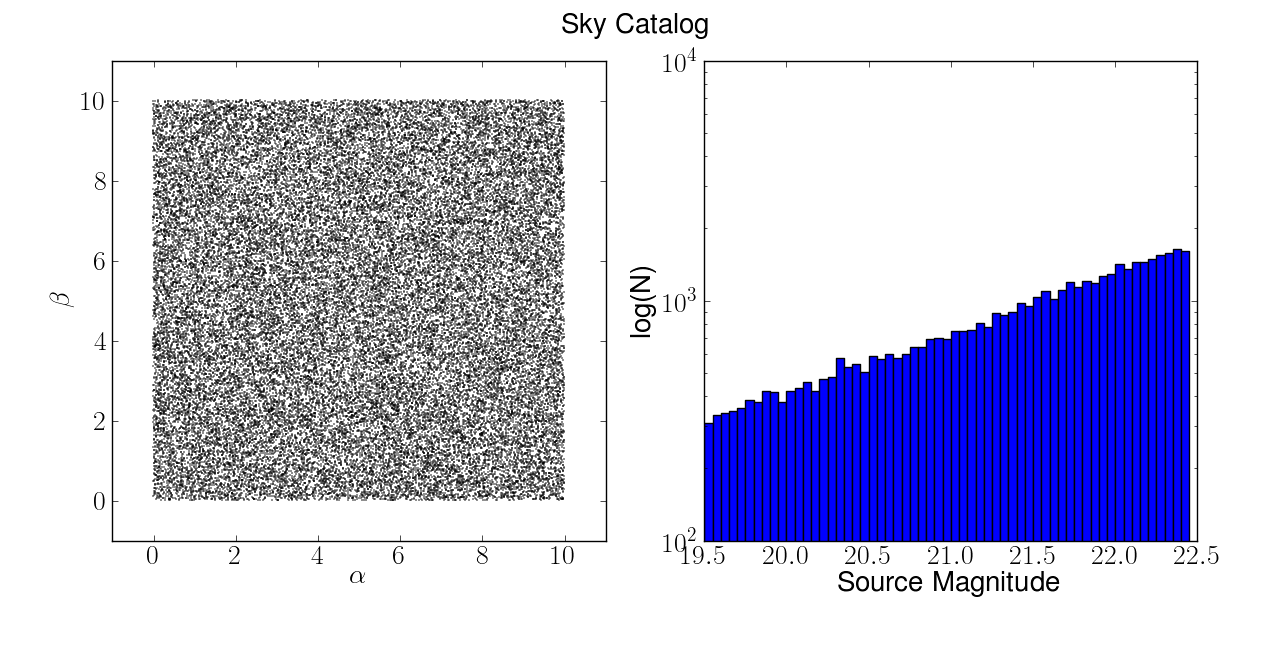
\includegraphics[width=\textwidth]{Catalog.png}
\end{center}
\caption{The catalog of fake stars. The stars are shown at their position on the sky (left) and as a histogram of their magnitudes (right).
\label{fig:sky}}
\end{figure}

We relate star magnitudes, $m$, to star fluxes, $s$, simply by:
\begin{displaymath}
m = 22.5 - 2.5\log_{10}(s)
\end{displaymath}
and therefore do not consider the NISP instrument's absolute response.

\section{Single Exposure}
With a given camera pointing $(\alpha, \beta)$ and camera orientation $(\theta)$, we transform the sky catalog into focal plane coordinates and find all the stars falling within the instrument's field-of-view. The NISP instrument's field-of-view of $0.7 \times 0.7$~deg$^{2}$ is used as the default in the simulations. We do not simulate images, instead we trivially convert the actual star fluxes into measured counts $(c)$ with a flat field model $(f)$ and a noise model. A typical exposure is depicted in Figure \ref{fig:camera}.

\begin{figure}[ht]
\begin{center}
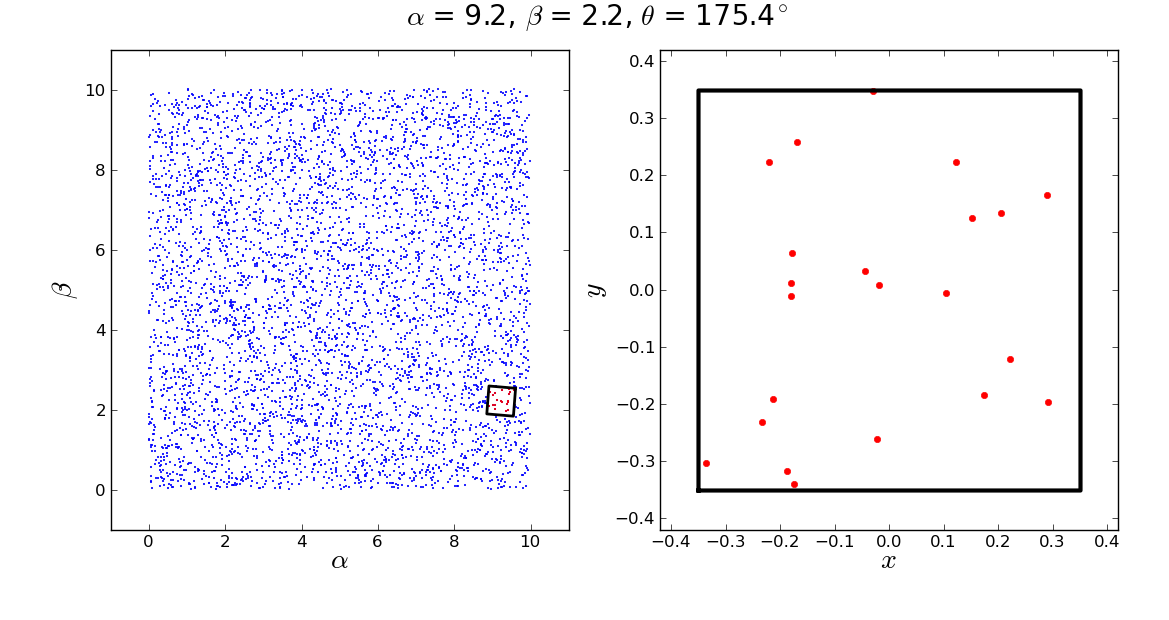
\includegraphics[width=\textwidth]{camera_image.png}
\end{center}
\caption{A single exposure of the sky with the pointing coordinates $(\alpha = 9.2^\circ, \beta = 2.2^\circ)$ and an orientation of $\theta = 175.4^\circ$. Left: Plot of the entire fake sky, with the instrument's field-of-view shown in black and the measured sources highlighted in red. Right: The distribution of the highlighted sources on the instrument's focal plane. \label{fig:camera}}
\end{figure}

\subsection{Catalog to Measured Counts Conversion}
For a measurement $(i)$ the counts recorded from a star (with an ID $k$) depends on God's flat-field ($f(\vec{q}_{god})$), which is a function of focal plane position $(\vec{x_i})$, and the star's true flux ($s$): 

\begin{displaymath}
c_i = f(\vec{x_i} | \vec{q}_{god}) . s_{k} + e_{i}
\end{displaymath}

\noindent{}An error, drawn from the Normal Distribution $N(e|0,{\sigma_i}^2)$, is also introduced to the measurement.

\subsection{Noise Model}
We assume that the Euclid exposures will be background limited and that, for systematic reasons, we will hit an upper limit on the signal-to-noise for bright sources. We assume that the uncertainty variance on the counts are:

\begin{displaymath}
\sigma_{{ass}}^{2} = \alpha^{2} + \eta^{2}\, c^{2} 
\end{displaymath}
\noindent{}where $\alpha$ and $\eta$ are both constants. In fact, we complicate the model by applying an extra term to the count's uncertainty variance, which we do not take into account in our analysis: 

\begin{displaymath}
\sigma_{{act}}^{2} = (1 + \epsilon) \,\alpha^{2} + \eta^{2}\, c^{2} 
\end{displaymath}
\noindent{}where $\epsilon$ is a random number, in the range [0.0, $\epsilon_{max}$), generated for each measurement $i$. The assumed and the actual uncertainty variances are shown in Fig. \ref{fig:count_uncertainty}.

\begin{figure}[ht]
\begin{center}
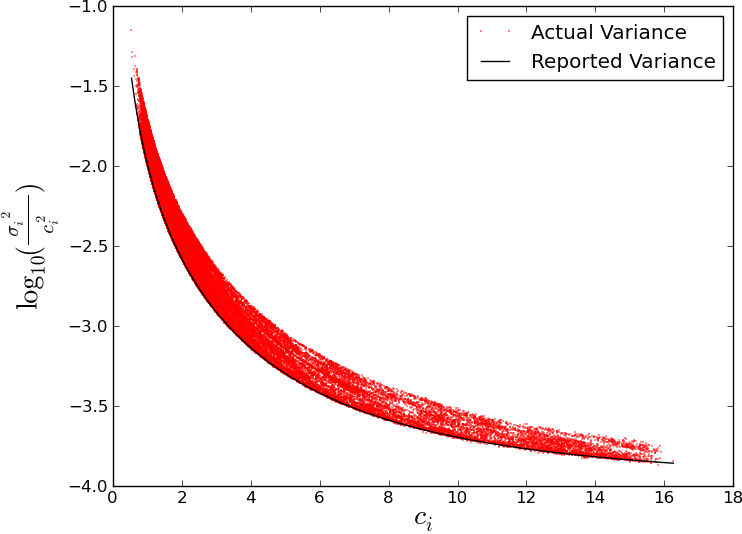
\includegraphics[width=\textwidth]{invvar_plot.png}
\end{center}
\caption{The assumed and the actual variances as a function of counts.\label{fig:count_uncertainty}}
\end{figure}

\section{Ubercalibration}
The ubercalibration procedure works in two sub-steps: (i) the star fluxes are refined based on the latest flat-field estimate (\textit{s\_step}) and (ii) the flat-field parameters are refined based on the latest star flux estimates (\textit{q\_step}). We iterate these steps until the parameters converge. Our flat-field is defined by a set of parameters $\vec{q}$. The individual star measurements are defined as $c_i$ (``counts''), where each $i$ corresponds to a exposure number $n$, a specific star (with ID number $k$) and a focal plane position $\vec{x}$.

Our model is

\begin{displaymath}
c_i = f(\vec{x_i} | \vec{q}) . s_{k} + e_{i}
\end{displaymath}

where $s_k$ is the true flux from star $k$ and our error is drawn from the Normal Distribution $e_{i} = N(e|0,{\sigma_i}^2)$.

\subsection{Star Flux Refinement: \textbf{\textit{s\_step}}}
The flux estimates, $s_k$, for each star can be considered individually. At each \textit{s\_step} we can refine a star's flux estimate by minimizing the error function with the latest flat-field parameters:

\begin{displaymath}
\chi^2_{k} = \sum_{i \in \mathcal{O}(k)} \frac{(c_i-f_{i}s_{k})^2}{{\sigma_i}^2}
\end{displaymath}

\begin{displaymath}
\frac{d\chi^2_{k}}{d s_{k}} = \sum_{i \in \mathcal{O}(k)} \frac{-2 f_{i} (c_i-f_{i}s_{k+1})}{{\sigma_i}^2} = 0
\end{displaymath}

\begin{displaymath}
s'_{k} \leftarrow \left[{\sum_{i \in \mathcal{O}(k)}  \frac{f_{i}^2}{{\sigma_i}^2}} \right]^{-1}  \left[ {\sum_{i \in \mathcal{O}(k)} \frac{f_{i} c_i}{{\sigma_i}^2}} \right]
\end{displaymath}

The standard uncertainty variance on the new star flux estimate, $s'_{k}$, is given by:

\begin{displaymath}
\sigma'^2_s = \left[{\sum_{i \in \mathcal{O}(k)}  \frac{f_{i}^2}{{\sigma_i}^2}} \right]
\end{displaymath}


\subsection{Flat-Field Refinement: \textbf{\textit{p\_step}}}
The flat-field parameters can now be refined with the latest star flux estimates. To do this we minimize the error function for all measurements with respect to the flat-field parameters.

\begin{displaymath}
\chi^2 = \sum_{i} \frac{(c_i-f_{i}s'_{k})^2}{{\sigma_i}^2}
\end{displaymath}

\begin{displaymath}
f_{i} = \sum_{l = 1}^L q_{lj} g_l(\vec{x_i})
\end{displaymath}

\begin{displaymath}
\chi^2 = \sum_{i} \frac{(c_i- s'_{k} \sum_{l = 1}^L q_{lj} g_l(\vec{x_i}))^2}{{\sigma_i}^2}
\end{displaymath}

\begin{displaymath}
\frac{d\chi^2}{dq_{lj}} = \sum_{i} \frac{-2 g_l(\vec{x_i}) s'_{k} (c_i- s'_{k} \sum_{l' = 1}^{L'} q_{l'} g_{l'}(\vec{x_i}))}{{\sigma_i}^2} = 0
\end{displaymath}

\begin{displaymath}
\sum_{i} \frac{g_l(\vec{x_i}) s'_{k} c_i}{{\sigma_i}^2} = \sum_{i} \frac{g_l (\vec{x_i}) s'^2_{k} \sum_{l' = 1}^{L'} q_{l'} g_{l'} (\vec{x_i})} {{\sigma_i}^2}
\end{displaymath}

\section{Initial Results}

\subsection{God's Flat Field}
We first consider the simple case where God's flat field is given by:
\begin{displaymath}
f(\vec{x} | \vec{q}) = 1 - 0.3\,x^2 - 0.5\,y^2 
\end{displaymath}

\subsection{Surveys Strategies}
We consider two extreme survey examples. The first, called Strategy A, consists of a regular grid of pointings over the sky with a small overlap between neighboring fields. Nine passes are performed over the sky and each time the grids are aligned exactly. The second survey, Strategy D, has the same number of fields as Strategy A, but the pointing and orientation of these fields are random. These two surveys can be seen in Fig. \ref{fig:surveys}.


\begin{figure}[ht]
\begin{center}
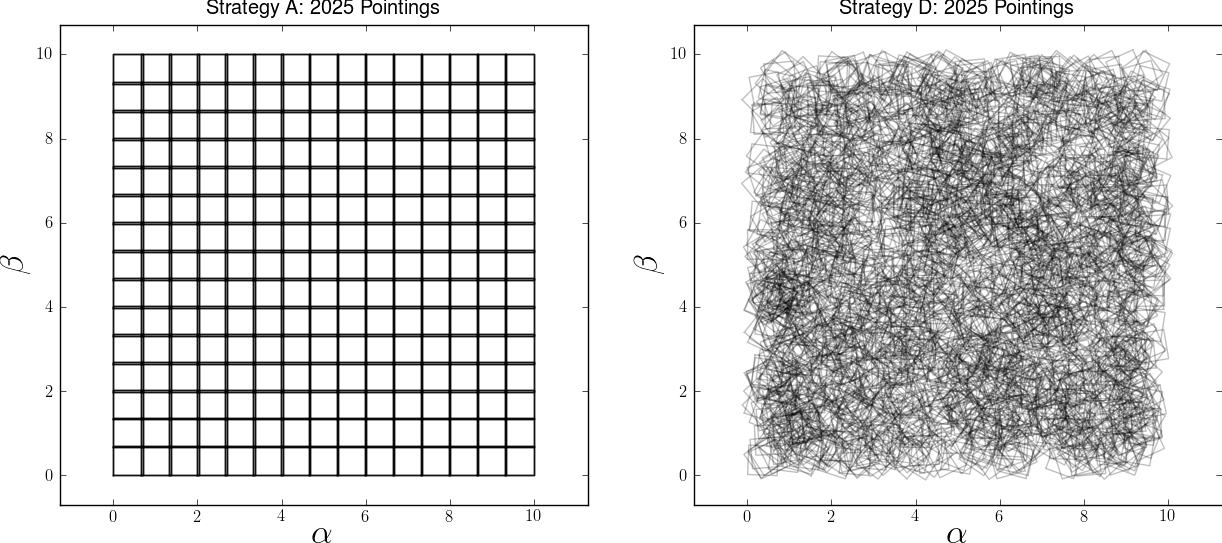
\includegraphics[width=\textwidth]{surveys.png}
\end{center}
\caption{Left: The A Strategy has regular pointings over the sky with a small overlap between adjacent fields. Nine passes are performed over the sky and each time the grids are aligned exactly. Right: The D Strategy has the same number of pointings as the A Strategy, but the pointings and orientations are random.\label{fig:surveys}}
\end{figure}

The coverage of each strategy is shown in Fig. \ref{fig:coverage}.

\subsection{Ubercalibration Performance}

The difference in ubercalibration method's ability to fit the flat field and the star magnitudes for the two different Strategies is striking. With the random Strategy (D) we can get very close to the actual flat field in a small number of ubercalibration iterations (see Fig \ref{fig:D}). The well ordered Strategy (A), on the other hand, does not converge to the correct flat field even with 1,000 ubercal iterations. Even when we start with almost the correct flat-field parameters (those found with the D Strategy - shown in Fig. \ref{fig:D}), the ubercalibration procedure does not converge. In fact, with each iteration solution drifts away from the actual flat-field. Fig \ref{fig:A} shows the fitted flat-field from Strategy A after 1,000 with the initial parameters shown in Fig \ref{fig:D}.

\begin{figure}[ht]
\begin{center}
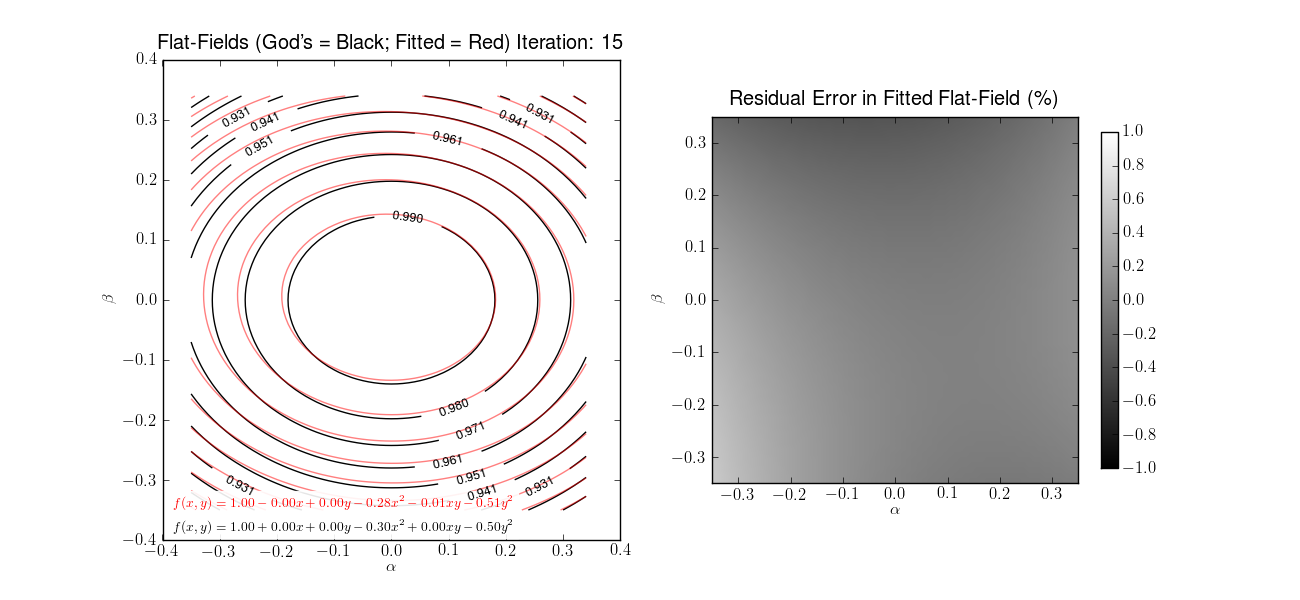
\includegraphics[width=\textwidth]{D_15_ff.png}
\end{center}
\caption{The fitted flat field compared to the actual flat field found with Strategy D. \label{fig:D}}
\end{figure}

\begin{figure}[ht]
\begin{center}
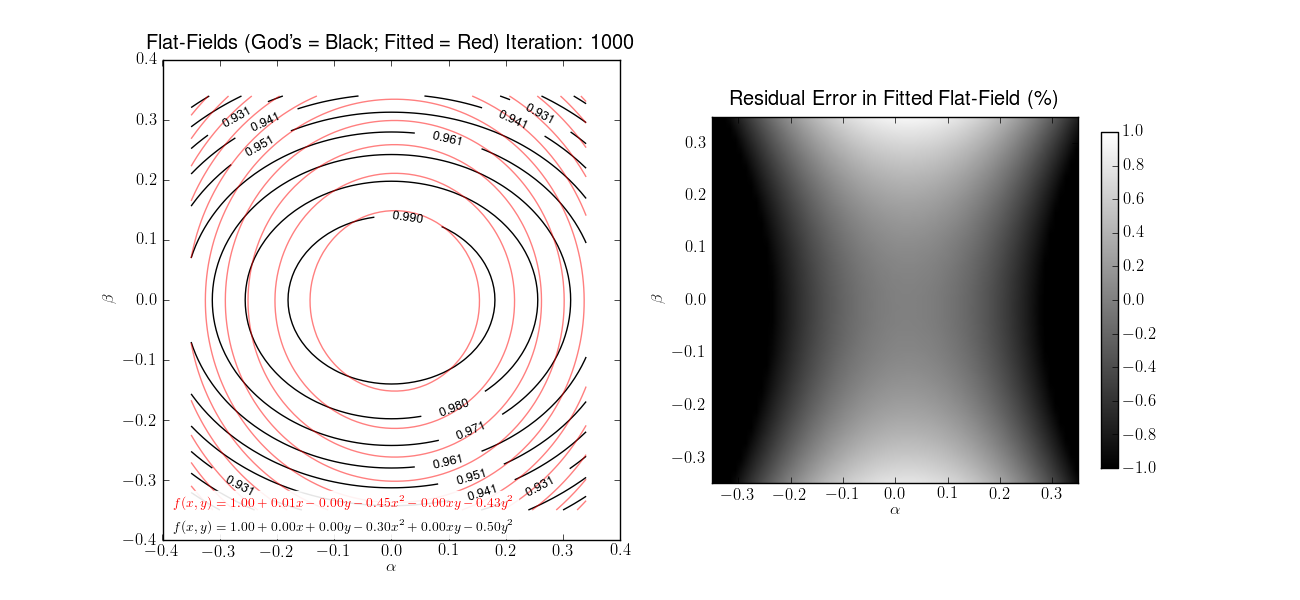
\includegraphics[width=\textwidth]{A_1000_ff.png}
\end{center}
\caption{The fitted flat field compared to the actual flat field calculated found with Strategy A. The ubercalibration procedure was started with almost exact flat field parameters (those found from Strategy D - see Fig. \ref{fig:D}) and has drifted away from the actual solution. \label{fig:A}}
\end{figure}

\begin{figure}[ht]
\begin{center}
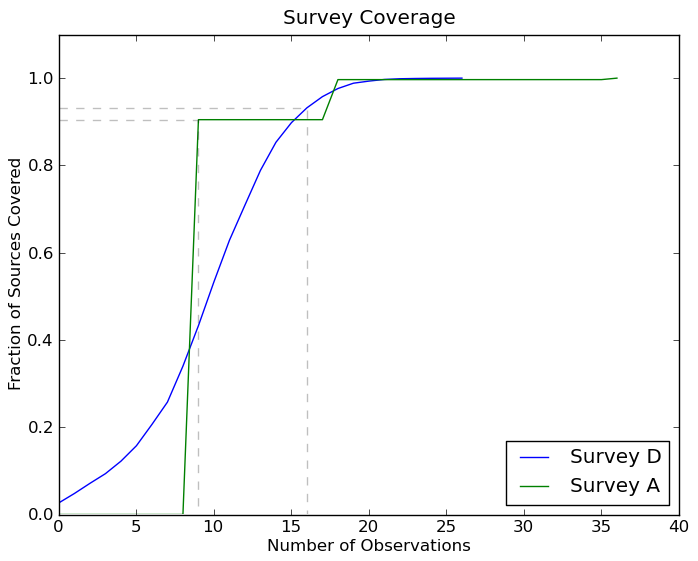
\includegraphics[width=0.47\textwidth]{coverage.png}
\end{center}
\caption{The coverage of both of the surveys investigated. \label{fig:coverage}}
\end{figure}

\end{document}
